\chapter{SVG and Vector Graphics Foundations}
\label{chap:svg_foundations}

\section{SVG as an input model for GPU conversion}

SVG is a declarative, XML-based language for 2D graphics \cite{w3c_svg2}.
Its main advantage is semantic richness: geometry, grouping, and styling are explicit in the source format.
For rendering systems, this means SVG provides high-level intent but not directly GPU-ready primitives.

In \texttt{Svg2GPU}, SVG is treated as a source description that must be transformed into typed geometry and style bundles.
This keeps authoring flexibility while enabling explicit rendering pipelines.

\section{Document semantics relevant to conversion}

A typical SVG document contains a root \texttt{<svg>} element, optional \texttt{viewBox}, primitive elements, and group containers.
For conversion, the most relevant subset is:

\begin{itemize}
\item \texttt{<path>} (general vector outlines),
\item \texttt{<rect>}, \texttt{<circle>}, \texttt{<ellipse>},
\item \texttt{<polygon>}, \texttt{<polyline>}, \texttt{<line>},
\item \texttt{<g>} for hierarchy.
\end{itemize}

Hierarchy is not a cosmetic detail.
Grouping affects inherited style and transform context, so flattening must preserve effective semantics.

\section{Path commands and geometric interpretation}

\subsection{Command classes}

Path data is encoded in the \texttt{d} attribute through command sequences:

\begin{itemize}
\item move commands: \texttt{M/m},
\item linear commands: \texttt{L/l}, \texttt{H/h}, \texttt{V/v},
\item curve commands: \texttt{C/c}, \texttt{S/s}, \texttt{Q/q}, \texttt{T/t},
\item arc commands: \texttt{A/a},
\item close command: \texttt{Z/z}.
\end{itemize}

Absolute and relative variants require parser state tracking (current point and subpath start).
Because path complexity dominates conversion effort, parser correctness here is foundational.

\subsection{Flattening and tolerance}

Curves and arcs generally require polyline approximation before triangulation.
A standard relation is:

\begin{equation}
\epsilon_{approx} \leq \tau,
\label{eq:svg_flattening_error}
\end{equation}

where $\epsilon_{approx}$ is approximation error and $\tau$ is tolerance.
Lower $\tau$ improves fidelity but increases vertex count and processing cost.

\section{Coordinate systems and transforms}

SVG conversion must preserve mapping across:

\begin{enumerate}
\item user space (SVG coordinates),
\item viewport/canvas space,
\item clip space for GPU rasterization.
\end{enumerate}

Transform handling is equally important.
Nested transforms are cumulative, and order matters.
With affine notation:

\begin{equation}
\mathbf{p'} = \mathbf{M}_{global} \cdot \mathbf{p},
\label{eq:svg_affine_mapping}
\end{equation}

where $\mathbf{M}_{global}$ is the accumulated transform matrix.

A practical architecture may either pre-transform geometry on CPU or apply transforms at draw time.
Either strategy is valid if applied consistently.

\subsection{ViewBox normalization as a conversion precondition}

In many SVG assets, the \texttt{viewBox} defines logical drawing coordinates that differ from physical output dimensions.
If this relation is ignored, valid geometry may appear clipped, scaled incorrectly, or displaced when rendered in canvas/WebGL space.
For this reason, conversion should normalize coordinates against the effective viewBox mapping before downstream geometry processing.

Let $(x_{min}, y_{min}, w_{vb}, h_{vb})$ be the viewBox and $(W, H)$ the target viewport.
A simplified normalization is:

\begin{equation}
x_{out} = \frac{x - x_{min}}{w_{vb}} \cdot W,\quad
y_{out} = \frac{y - y_{min}}{h_{vb}} \cdot H.
\label{eq:viewbox_normalization}
\end{equation}

Real implementations also account for preserve-aspect-ratio policy, but even this compact relation shows why coordinate conversion must happen explicitly and early.

\section{Style semantics and normalization}

For GPU-oriented conversion, style values must be canonicalized.
Relevant fields include:

\begin{itemize}
\item fill and fill opacity,
\item stroke, stroke width, stroke opacity,
\item line join/cap,
\item visibility/display,
\item fill rule (\texttt{nonzero}, \texttt{evenodd}).
\end{itemize}

Color parsing must normalize common authoring formats (HEX, RGB/A, HSL/A, named) into numeric RGBA form \cite{mdn_svg}.
Normalization early in the pipeline simplifies geometry and renderer logic.

\subsection{Fill-rule implications}

Fill rules such as \texttt{nonzero} and \texttt{evenodd} are critical for compound paths and nested contours.
If conversion ignores this distinction, generated interiors can be topologically incorrect.
For this reason, fill-rule interpretation should be carried as explicit metadata and resolved before triangulation.

\subsection{Opacity composition}

In practical rendering, element opacity and channel opacity should be combined deterministically.
A useful relation is:

\begin{equation}
\alpha_{effective} = \alpha_{channel} \cdot \alpha_{element}.
\label{eq:alpha_effective}
\end{equation}

This avoids inconsistent alpha behavior between fill and stroke processing paths.

\section{From SVG semantics to conversion requirements}

\begin{table}[htbp]
\centering
\caption{Semantic-to-implementation requirements}
\label{tab:svg_semantic_requirements}
\begin{tabular}{>{\raggedright\arraybackslash}p{4.0cm} >{\raggedright\arraybackslash}p{4.8cm} >{\raggedright\arraybackslash}p{4.6cm}}
\toprule
\textbf{Semantic area} & \textbf{Risk if ignored} & \textbf{Required behavior} \\
\midrule
Path syntax and parameters & invalid geometry or parser failure & strict command/token validation \\
Fill rule semantics & wrong interior regions & winding-aware fill handling \\
Transform hierarchy & spatial mismatch & cumulative transform consistency \\
Style normalization & inconsistent visual output & canonical numeric style model \\
Visibility/display flags & unnecessary processing & early element filtering \\
\bottomrule
\end{tabular}
\end{table}

This mapping is central to architecture decisions in later chapters.
It defines what must be guaranteed before geometry generation starts.

\subsection{Supported-semantic policy}

An engineering thesis cannot cover the full SVG recommendation at implementation level.
Therefore, a practical semantic policy is required:

\begin{itemize}
\item \textbf{fully supported semantics:} path syntax, common primitives, core fill/stroke attributes, and transform accumulation;
\item \textbf{partially supported semantics:} complex edge combinations requiring stricter triangulation assumptions;
\item \textbf{deferred semantics:} advanced filters, full text layout, and effect stacks outside current scope.
\end{itemize}

This policy improves both correctness and communication.
Correctness improves because unsupported cases are identified explicitly instead of failing unpredictably.
Communication improves because limitations are documented as deliberate scope boundaries rather than hidden defects.

\section{Illustrative project examples}

Two project examples illustrate these concepts.
The first is a controlled basic geometry scene used for sanity checks.
The second is a complex SVG input used as stress case.

\begin{figure}[htbp]
    \centering
    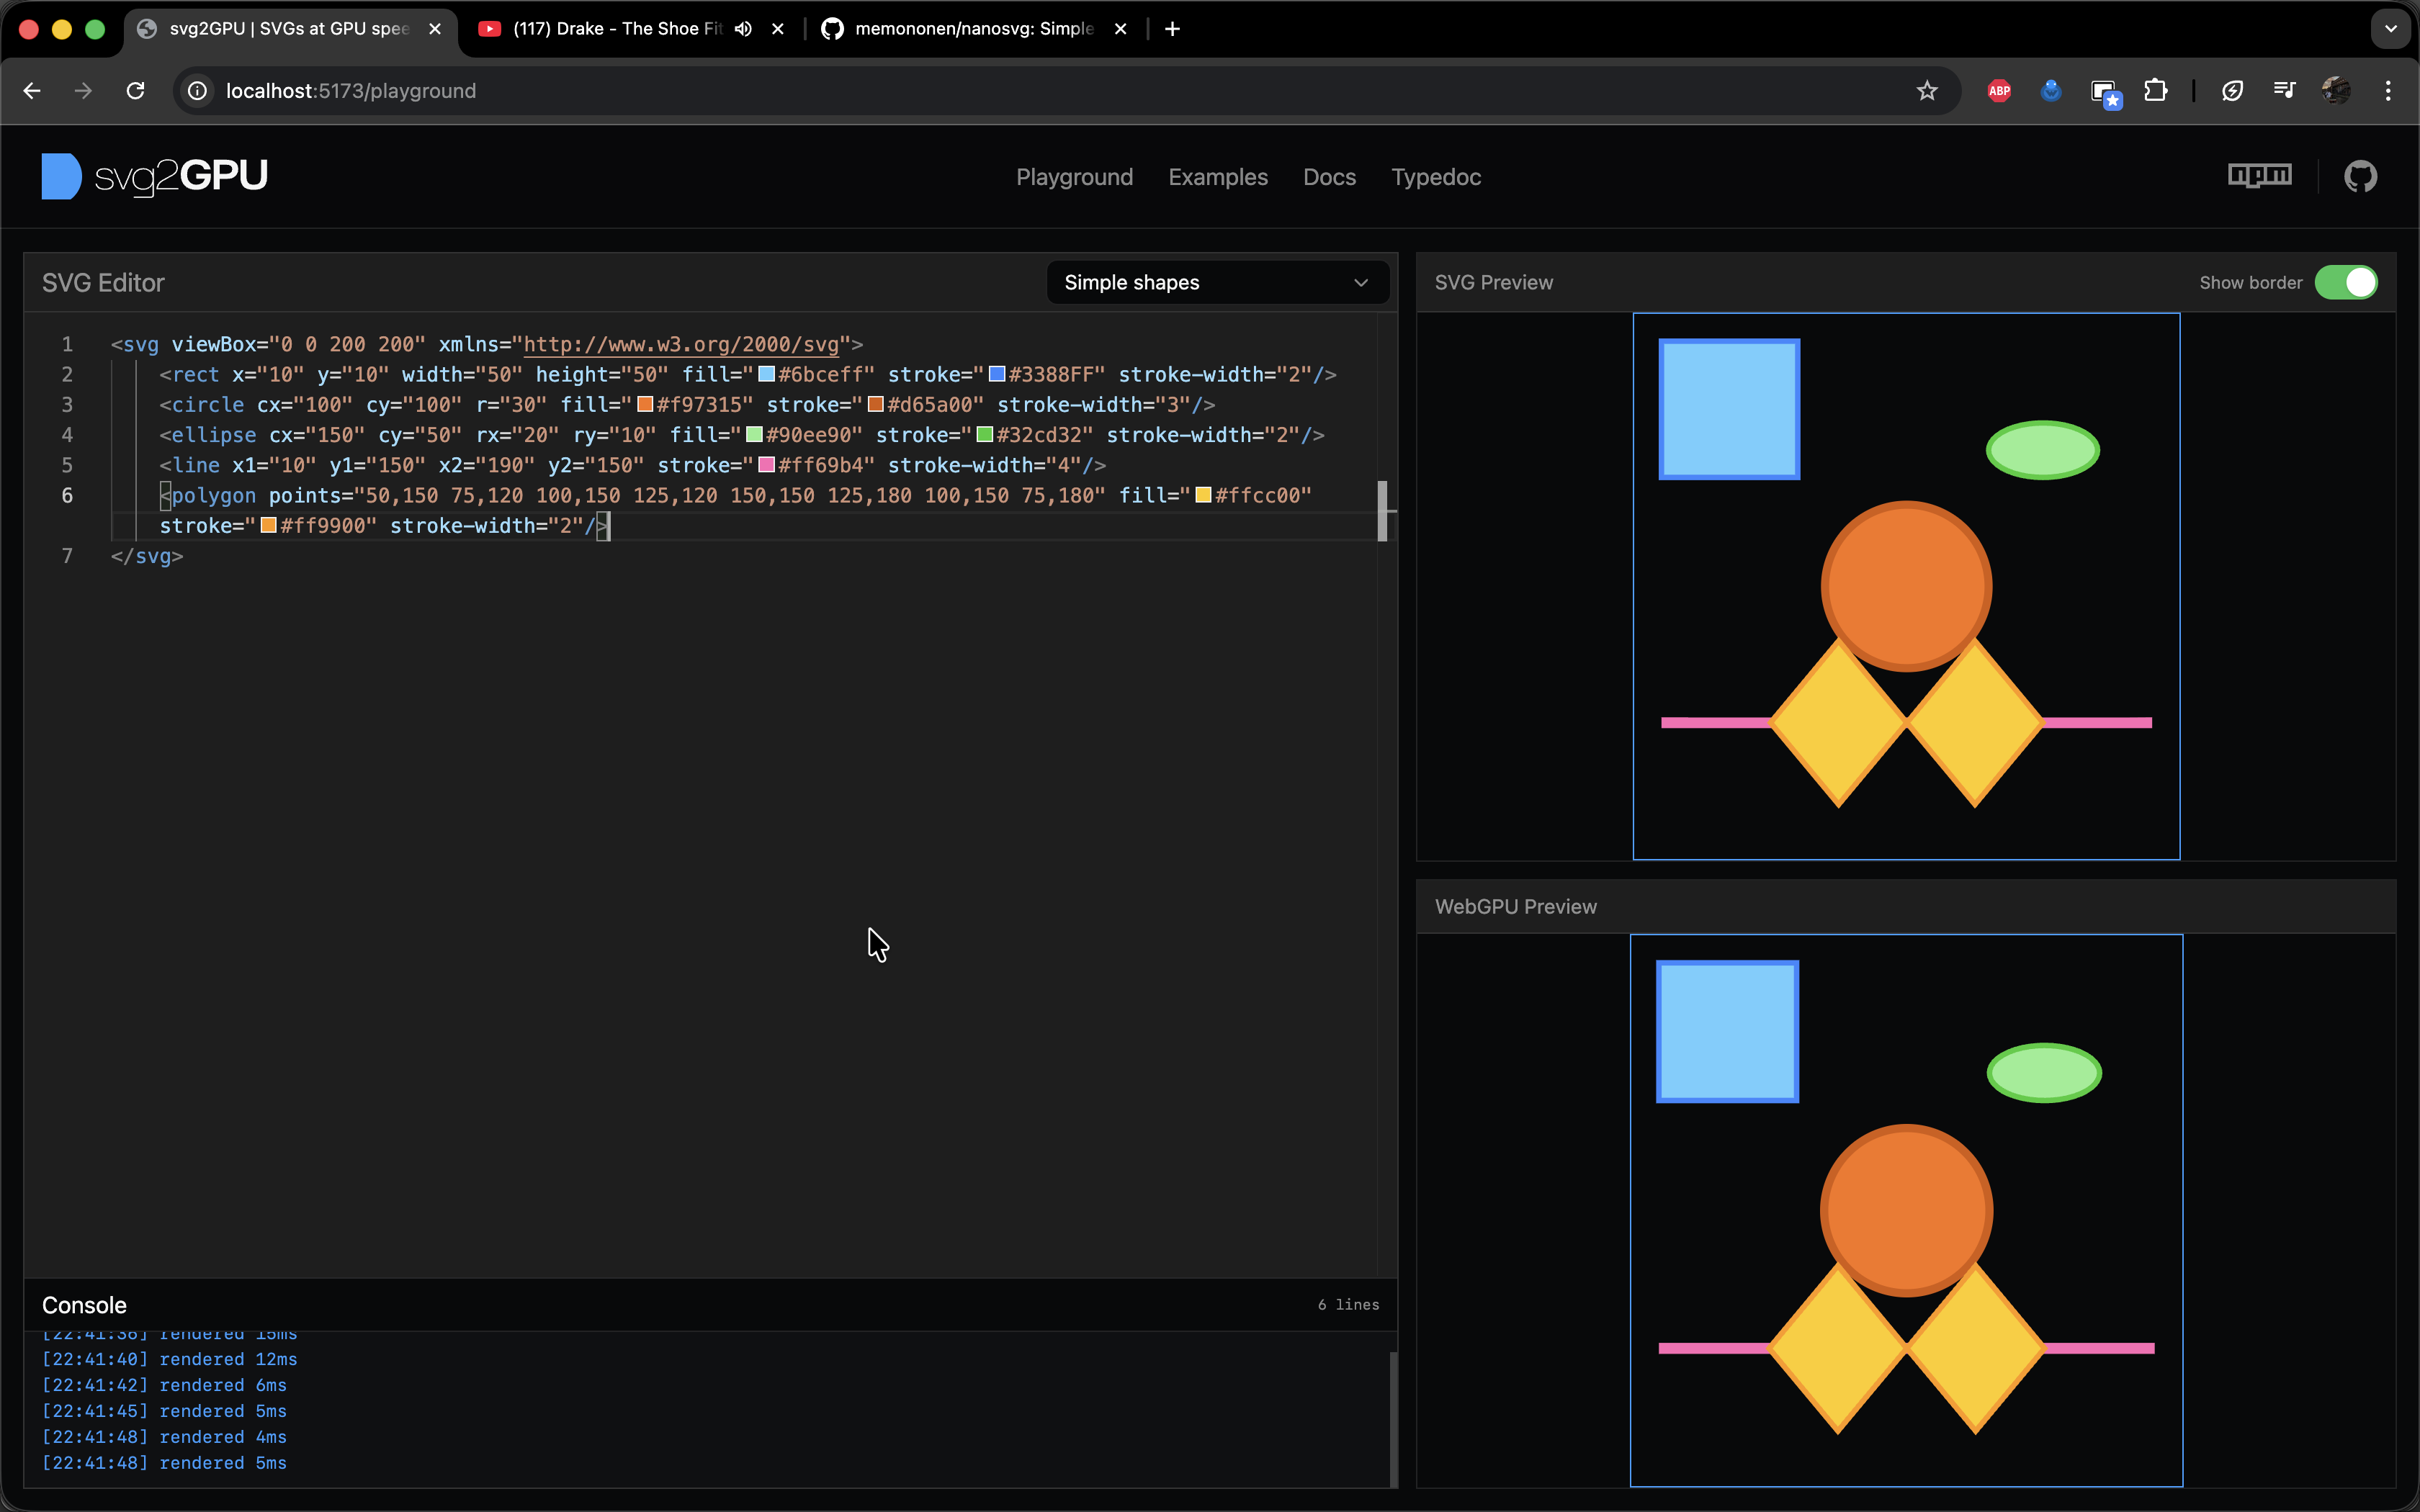
\includegraphics[width=0.92\textwidth]{figures/BasicGeometries.png}
    \caption{Basic geometry example used for parser and style sanity checks}
    \label{fig:svg_basic_example}
\end{figure}

\begin{figure}[htbp]
    \centering
    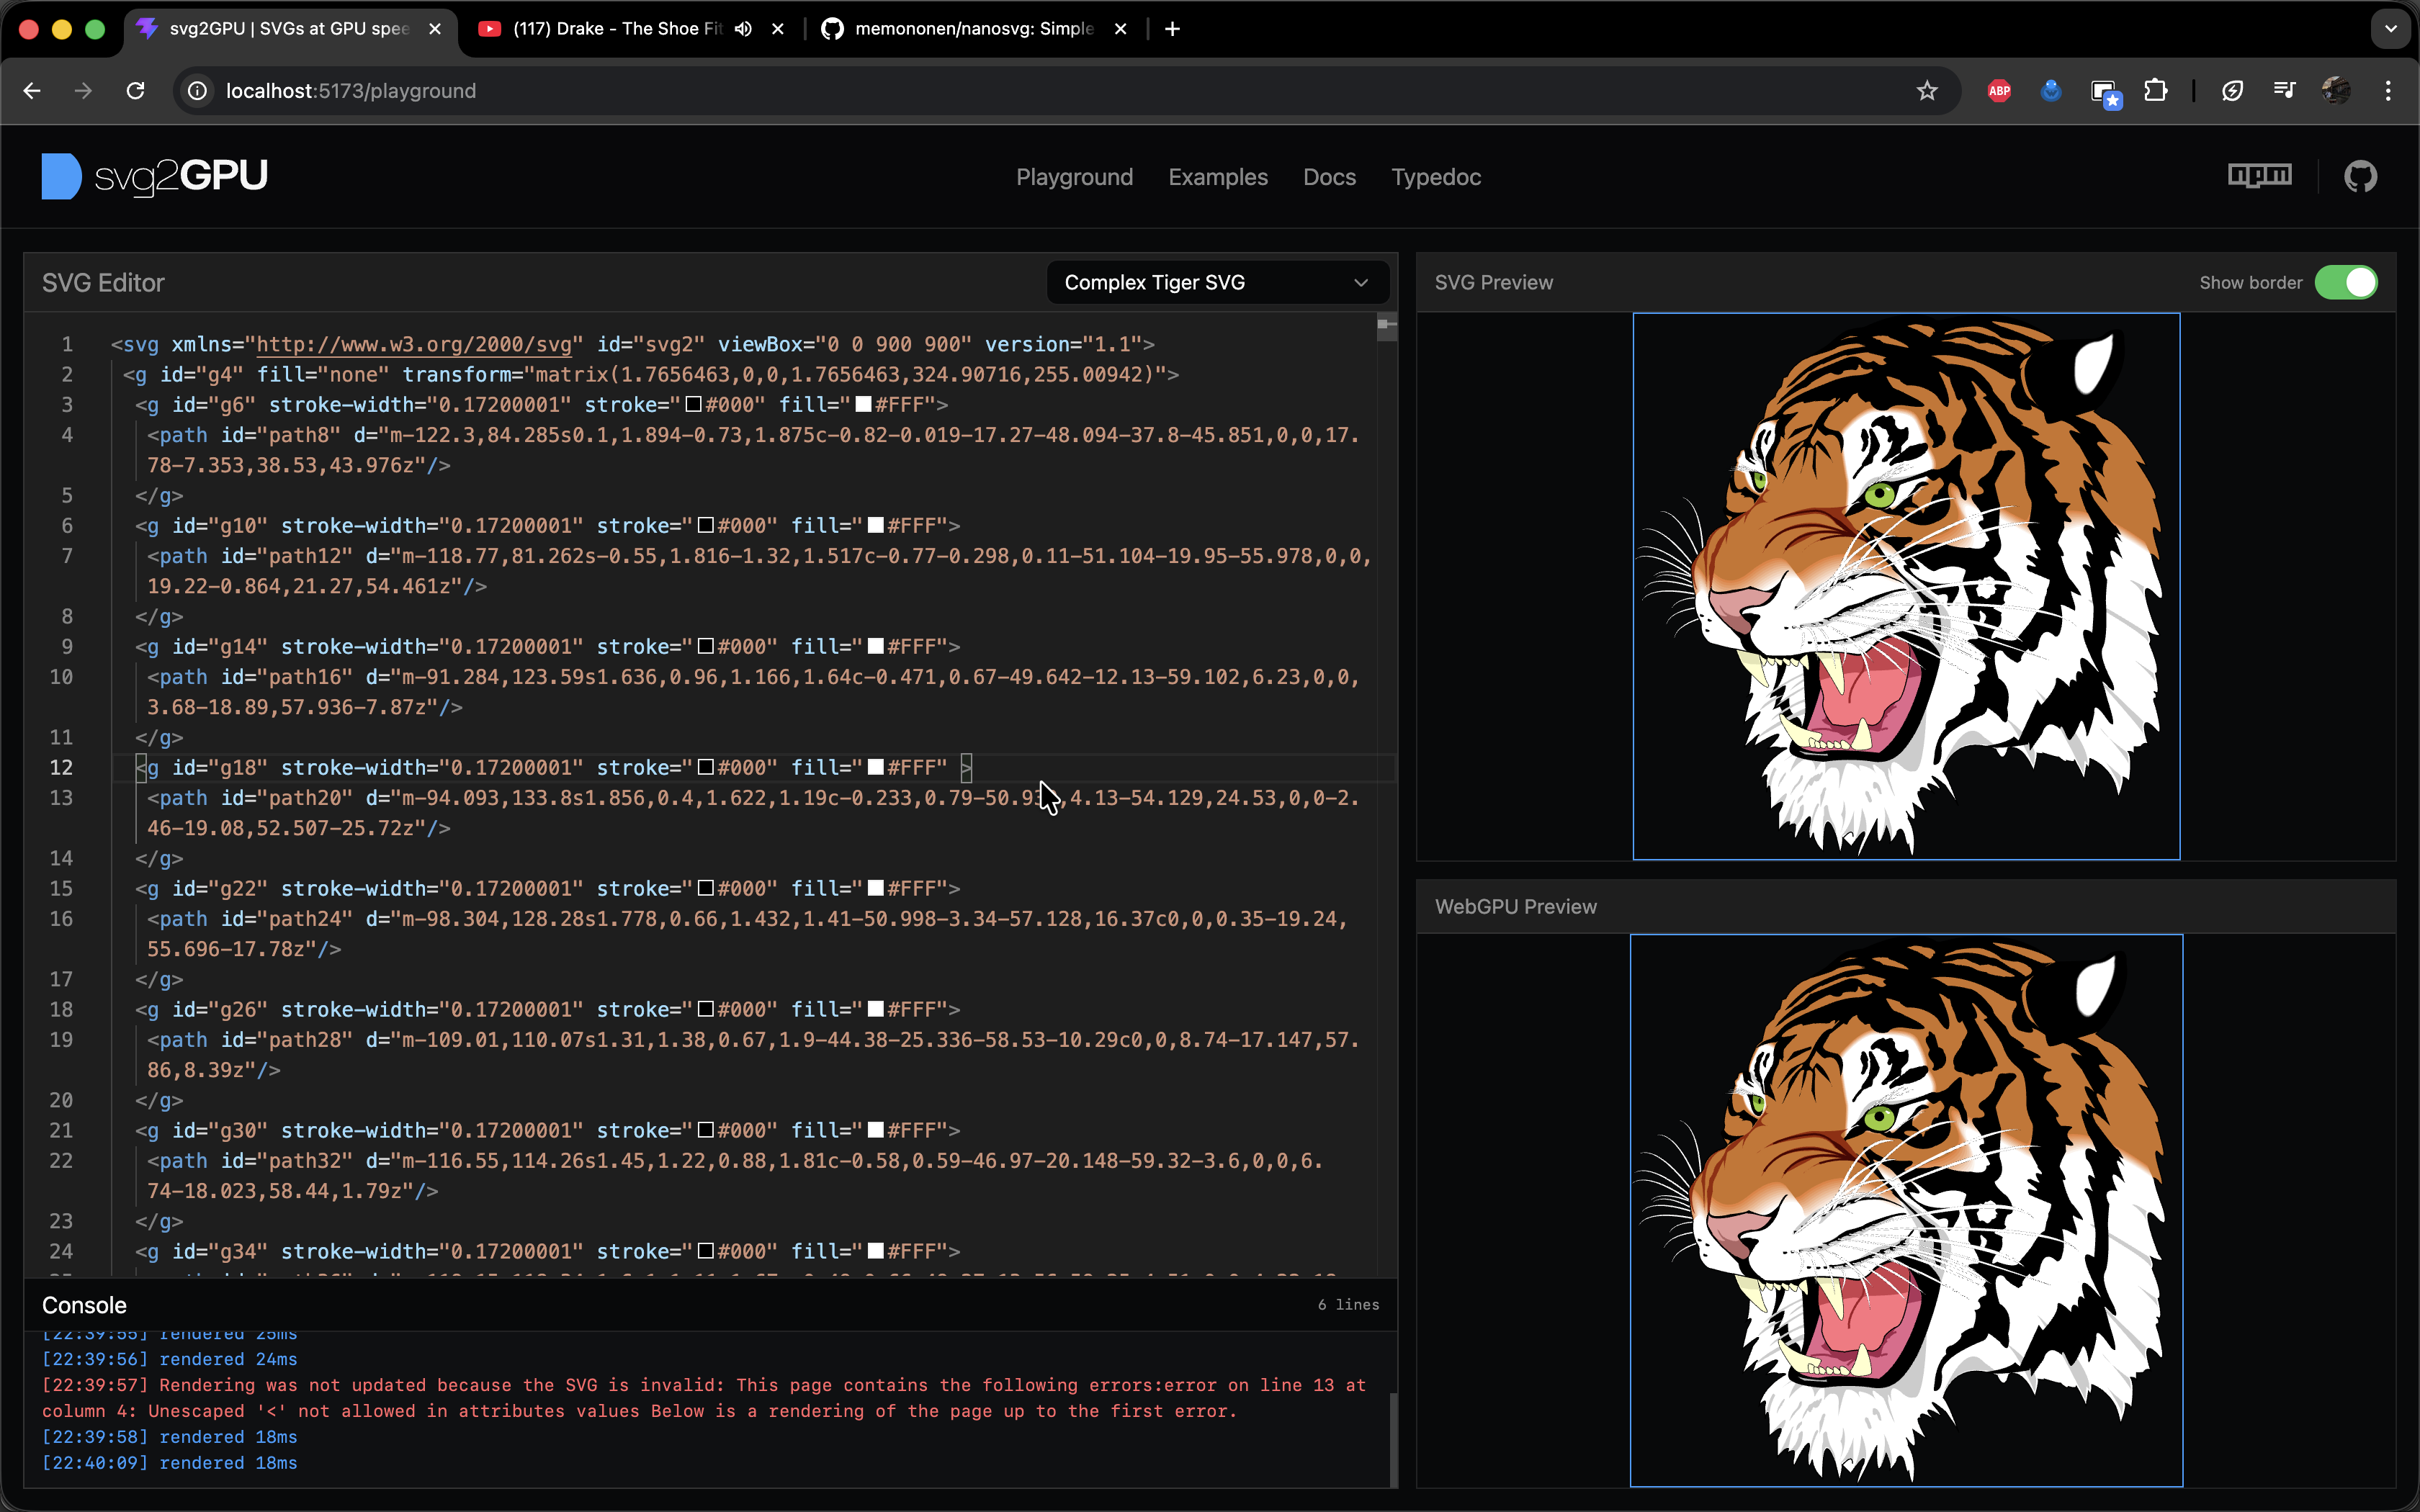
\includegraphics[width=0.92\textwidth]{figures/TigerSVG.png}
    \caption{Complex SVG stress case used for robustness observation}
    \label{fig:svg_complex_example}
\end{figure}

The controlled case validates expected behavior quickly.
The complex case reveals robustness limits and conversion edge conditions.

\section{Positioning among browser graphics models}

SVG differs from immediate-mode APIs (Canvas, WebGL draw loops) because it retains scene semantics.
This is excellent for authoring but requires conversion for explicit GPU pipelines.
In other words:

\begin{itemize}
\item SVG defines what the scene means,
\item GPU APIs define how primitives are processed.
\end{itemize}

\texttt{Svg2GPU} is positioned precisely at this boundary.
The parser and geometry layers translate semantic structure into explicit draw-ready data.

\subsection{Maintainability impact of layer separation}

Separating parser semantics, geometry conversion, and rendering reduces coupling.
This enables targeted testing and controlled evolution of each layer.
For example, triangulation changes can be introduced without modifying XML parsing logic, and renderer optimization can proceed without changing command parsing contracts.

\subsection{Why this foundation matters for later implementation chapters}

The concepts introduced here are not only theoretical background.
They directly constrain implementation order and module responsibilities:

\begin{itemize}
\item command semantics determine parser contract shape;
\item transform and viewBox rules determine coordinate preprocessing;
\item fill-rule semantics constrain triangulation behavior;
\item style normalization determines renderer input stability.
\end{itemize}

When these foundations are explicit, architecture decisions can be justified by requirements instead of personal coding preference.
This makes the practical part of the thesis more reproducible and easier to evaluate.

\section{Chapter summary}

This chapter established the semantic foundations required by the rest of the thesis:

\begin{itemize}
\item SVG is semantically rich but not directly GPU-native.
\item Path and style interpretation dominate conversion complexity.
\item Coordinate and transform consistency is mandatory for correctness.
\item Fill-rule and style normalization are core requirements, not optional details.
\item A robust conversion system must combine strict validation with practical fallback behavior.
\end{itemize}

These foundations lead naturally to the next chapter, which focuses on geometry processing strategy and algorithmic trade-offs for vector-to-mesh conversion.
